% =======================================================================
\section{Results}

\subsection{Connected components (\texorpdfstring{$H_0$}{})}
\label{sec:scaleh0}

Throughout, $H_0$ is the number of cluster centroids. Equivalently, it
is $\beta_0$ of the Vietoris--Rips complex on those centroids at
filtration zero. Primary-match figures come from the uniform 150-frame
sample of match 1996435 (Section~\ref{sec:data}). Ten-match aggregates
use the same sampling scheme (1{,}500 frames in total).

At the individual level ($\delta = 2.75$~m),
$H_0 = 19.32 \pm 2.34$ (mean $\pm$ s.d.; range 10--22). At the tactical
level ($\delta = 11.75$~m), $H_0 = 5.04 \pm 1.69$ (range 2--10). At the
team level ($\delta = 23.0$~m), the cloud usually collapses to one or
two clusters: mean $1.96 \pm 0.36$. All 22 players lie in a single
cluster in 8.7\% of frames, split across two in 86.7\%, and across
three in 4.7\%.

The same three-level pattern holds in all ten matches. Grand means are
individual $H_0 = 19.31 \pm 0.31$, tactical $H_0 = 5.09 \pm 0.38$, and
team cluster count $1.98 \pm 0.06$ (mean $\pm$ s.d.\ across matches).
Every match stays within the validated $H_0$ bands of
Section~\ref{sec:cutoffselection}. Figure~\ref{fig:cutoff} records the
sweep from which those cutoffs were taken.

\subsection{\texorpdfstring{$H_1$}{} loop detection}
\label{sec:h1detection}

On the primary match, the pipeline detects 403 $H_1$ loops across 150
uniformly sampled frames (Table~\ref{tab:h1single}). Loops at the
individual level are frequent and short-lived. They appear in 144 of
150 frames (96.0\%), at a mean rate of 2.52 per frame, with low mean
persistence ($1.974 \pm 1.118$~m). Loops at the tactical level are
rarer but last longer: 23 frames (15.3\%), mean rate 0.17 per frame,
mean persistence $3.914 \pm 2.745$~m, maximum 10.771~m. Loops at the
team level never occur ($H_1 = 0$ across all 1{,}500 frames in the
ten-match sample).

Table~\ref{tab:h1single} collects these statistics in compact form.
$F$ denotes the fraction of frames with at least one loop; L/f, the
mean loop count per frame; $\bar{p}$, mean persistence (death minus
birth, in metres); and $p_{\max}$, maximum persistence.

\begin{table}[h]
\centering
\caption{Single-match \texorpdfstring{$H_1$}{} statistics (primary match, 150 frames).}
\label{tab:h1single}
\begin{tabular}{@{}lccccr@{}}
\toprule
Level & Total & $F$ (\%) & L/f & $\bar{p}$ (m) & $p_{\max}$ (m) \\
\midrule
Individual (2.75~m) & 378 & 144/150 (96.0\%) & 2.52 & $1.974\pm1.118$ & 12.991 \\
Tactical (11.75~m)  & 25  & 23/150 (15.3\%)  & 0.17 & $3.914\pm2.745$ & 10.771 \\
Team (23.0~m)       & 0   & 0/150 (0\%)      & N/A  & N/A             & N/A \\
\bottomrule
\end{tabular}
\end{table}

\begin{remark}[Team-level $H_1$ vanishes a priori]
\label{rem:teamnull}
At $\delta = 23.0$~m the 22 players reduce to $k\le 2$ centroids in
93.6\% of complete frames on the ten-match sweep
(Section~\ref{sec:cutoffselection}). A Vietoris--Rips complex on at
most two points cannot carry a non-trivial 1-cycle. Frames with $k=3$
are 6.4\% of that sweep; they are the only team-level configurations
in which a loop is possible. Our headline $H_1$ analysis therefore
runs at two levels (individual and tactical) against the three-level
$H_0$ decomposition above. Team-level loop structure on the typical
envelope would require a different representation (density fields or
Delaunay triangulations, for example).
\end{remark}

The two-level $H_1$ pattern extends to all ten matches (1{,}500
uniformly sampled frames; Table~\ref{tab:h1multi}). Individual-level
presence is $96.5\%\pm1.5\%$ (95\% CI $95.6$--$97.3\%$), between 94.7\%
and 98.7\% in every match. Tactical presence is $18.8\%\pm6.5\%$ (95\%
CI $15.2$--$22.7\%$), ranging from 11.3\% to 31.3\% across matches. The
primary match (15.3\% tactical) sits within one standard deviation of
the ten-match mean. That match was chosen for broadcast quality and
event annotation, not for its tactical $H_1$ rate.

Table~\ref{tab:h1multi} reports the same quantities across ten matches;
s.d.\ denotes the standard deviation of each quantity across matches.

\begin{table}[h]
\centering
\caption{Multi-match \texorpdfstring{$H_1$}{} statistics (10 matches). Presence = mean \texorpdfstring{$\pm$}{} s.d.\ across matches; 95\% bootstrap CIs from 1{,}000 resamples over matches.}
\label{tab:h1multi}
\begin{tabular}{@{}lccccr@{}}
\toprule
Level & Total & Presence (\%) & 95\% CI & $\bar{p}$ (m) & s.d. \\
\midrule
Individual & 4{,}039 & $96.5\%\pm1.5\%$ & $95.6$--$97.3\%$ & 1.885 & 0.149 \\
Tactical   & 306     & $18.8\%\pm6.5\%$ & $15.2$--$22.7\%$ & 0.647 & 0.229 \\
Team       & 0       & $0.0\%\pm0.0\%$  & N/A              & N/A   & N/A \\
\bottomrule
\end{tabular}
\end{table}

Mean $\bar{p}$ in Table~\ref{tab:h1multi} averages over all sampled
frames, including those with no loop. The tactical entry is therefore
lower than the primary-match mean in Table~\ref{tab:h1single}, which is
taken only where loops appear.

Remark~\ref{rem:teamnull} explains why $H_1$ vanishes when clustering
leaves at most three centroids. The tactical level sits close to that
floor. In the ten-match sample, 40.6\% of frames have four or fewer
tactical centroids, and none of them carries a loop. Presence rate
alone cannot tell arrangement from cluster count. We separate the two
with the matched null of Section~\ref{sec:stats}, which fixes centroid
number and spatial envelope and randomises only arrangement.

Table~\ref{tab:null} summarises the result. Tactical observed presence
is more than twice the null rate. Table~\ref{tab:nullk} splits by
centroid count $k$. Presence is zero at $k\le 4$, as expected. It then
rises from 9.3\% at $k=5$ to 67.0\% at $k=8$, always above the null.
At the individual level the null already exceeds 91\%: twenty points
in a bounded region almost always close a cycle. The observed excess is
therefore modest ($+5.1$~pp). Tactical $H_1$ exceeds the null once
$k \ge 5$. Individual presence is already high under the null.

\begin{table}[h]
\centering
\caption{\texorpdfstring{$H_1$}{} presence against a cardinality- and envelope-matched null (10 matches, 1{,}500 frames, 200 null replicates per frame). Excess is in percentage points, with 95\% bootstrap CIs over matches.}
\label{tab:null}
\begin{tabular}{@{}lcccc@{}}
\toprule
Level & Observed & Null & Excess & 95\% CI \\
\midrule
Individual & 96.5\% & 91.4\% & $+5.1$ & $[+3.9, +6.1]$ \\
Tactical   & 18.8\% & 9.1\%  & $+9.7$ & $[+7.3, +12.2]$ \\
\bottomrule
\end{tabular}
\end{table}

\begin{table}[h]
\centering
\caption{Tactical-level \texorpdfstring{$H_1$}{} presence by centroid count \texorpdfstring{$k$}{}, against the matched null of Table~\ref{tab:null} (10 matches, 1{,}500 frames).}
\label{tab:nullk}
\begin{tabular}{@{}rcccc@{}}
\toprule
$k$ & Frames & Observed & Null & Excess \\
\midrule
$\le 4$ & 609 & $0.0\%$ & $0.4\%$ & $-0.4$ \\
5 & 344 & $9.3\%$ & $4.1\%$ & $+5.2$ \\
6 & 252 & $26.6\%$ & $12.0\%$ & $+14.5$ \\
7 & 149 & $51.0\%$ & $21.7\%$ & $+29.3$ \\
8 & 94 & $67.0\%$ & $33.4\%$ & $+33.6$ \\
$\ge 9$ & 52 & $84.6\%$ & $49.0\%$ & $+35.6$ \\
\bottomrule
\end{tabular}
\end{table}

\subsection{Closed cycle structures}

All 403 primary-match $H_1$ features receive a geometric realisation
via closed-cycle identification. The representative is the graph-cycle
proxy of Section~\ref{sec:cycles}, not a generator from the reduction
matrix. Cycles at the individual level form short rings of centroids
(typically three to six nodes in the examples we inspected). Tactical
cycles are similarly small (often four or five nodes) but span larger
gaps and persist longer. Figure~\ref{fig:cycles} shows the same sample
frame at both levels, with the cutoff and the filtration drawn as
separate panels (sample frame~95). The left column is the vertex set
after clustering. The right column is the longest-lived
\texorpdfstring{$H_1$}{} cycle on that set.
At \texorpdfstring{$\delta=2.75$}{}~m the vertices are four nearby
players and the cycle edges are $17.8$--$19.2$~m
(\texorpdfstring{$p=6.540$}{}~m).
At \texorpdfstring{$\delta=11.75$}{}~m the vertices are four groups,
one of them a $14$-player single-linkage cluster, and the cycle edges
are $21.1$--$28.8$~m (\texorpdfstring{$p=9.942$}{}~m).
The two cycles are not the same bar at two resolutions.
The persistence maxima in Table~1 are not used for the figure: the
individual-level maximum (frame~141) is a near-collinear sliver.

\begin{figure}[tp]
\centering
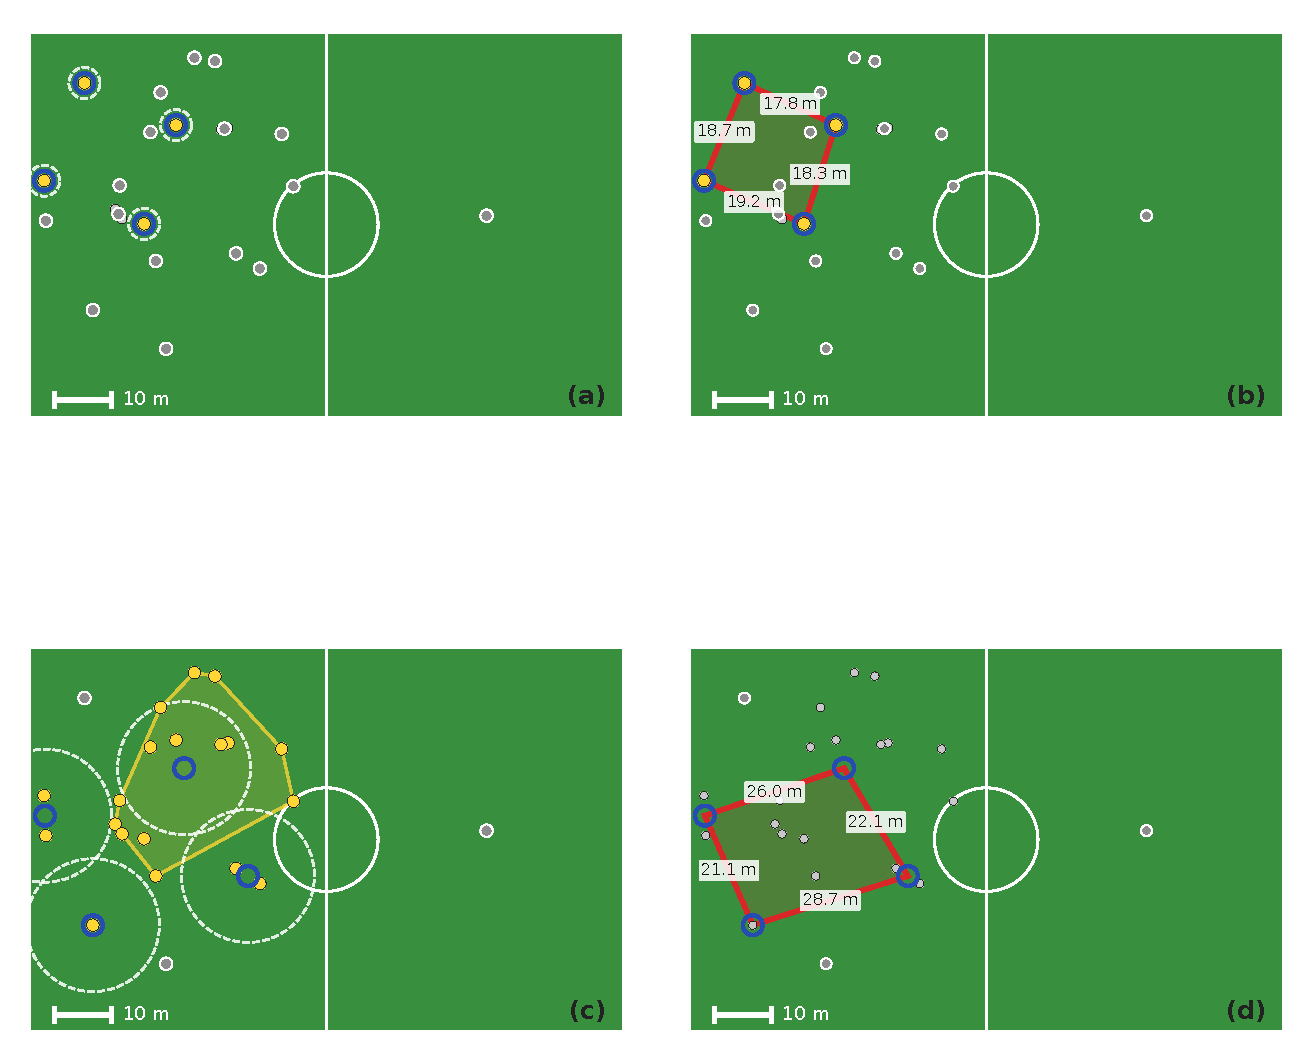
\includegraphics[width=\textwidth,keepaspectratio]{figures/fig3_cycle_geometry}
\caption{Cutoff versus filtration on one sample frame of SkillCorner
match 1996435 (sample frame~95). Left: vertex set after clustering at
\texorpdfstring{$\delta$}{}. Gold markers belong to this row's cycle
clusters; the hull in (c) is the 14-player single-linkage cluster;
dashed circles have radius \texorpdfstring{$\delta$}{} on the cycle
vertices only. Right: longest-lived \texorpdfstring{$H_1$}{}
representative on those vertices
(\texorpdfstring{$p=6.540$}{}~m and
\texorpdfstring{$p=9.942$}{}~m). Cycle edges are filtration
distances (\texorpdfstring{$17.8$--$19.2$}{}~m in (b);
\texorpdfstring{$21.1$--$28.8$}{}~m in (d)), not the cutoff.
Panel (d) draws centroids, not the absorbed players.
Compact four-cycles at both levels, not the persistence maximum.
A 10~m scale bar is shown on each panel. Uniform sample,
\texorpdfstring{$n=150$}{} frames, every 290th complete frame (the
same rule as the ten-match analysis).}
\label{fig:cycles}
\end{figure}

\subsection{Complementarity of the two \texorpdfstring{$H_1$}{} levels}
\label{sec:complementarity}

The two $H_1$ levels carry related but largely distinct information.
Over 1{,}500 uniformly sampled frames, total individual and tactical
$H_1$ persistence correlate weakly (Spearman $\rho=0.234$, $p<0.001$;
95\% bootstrap CI $[0.181, 0.276]$). The same holds for loop counts
($\rho=0.205$, $p<0.001$). The finding does not depend on how
persistence is summarised.

Co-occurrence exceeds chance (Fisher odds ratio 6.12, $p=0.002$;
bootstrap CI $[2.32, 16.33]$). Table~\ref{tab:fisher} shows the
asymmetry: 1{,}167 frames carry individual loops without a tactical
partner, and only two frames do the reverse. Weak rank correlation
remains the main evidence for complementarity. Joint presence need not
mean the two levels measure the same structure.

\begin{table}[h]
\centering
\caption{Frame counts of \texorpdfstring{$H_1$}{} presence at the two levels (1{,}500 frames).}
\label{tab:fisher}
\begin{tabular}{@{}lcc@{}}
\toprule
 & Tactical $H_1$ present & Tactical $H_1$ absent \\
\midrule
Individual $H_1$ present & 280 & 1{,}167 \\
Individual $H_1$ absent  & 2   & 51 \\
\bottomrule
\end{tabular}
\end{table}

A TDA-native check agrees. Bottleneck distance between the two levels'
diagrams has median 1.456~m and 95th-percentile tail 3.556~m. That is
on the order of typical tactical loop size on the primary match
(3.914~m mean persistence where loops appear;
Table~\ref{tab:h1single}). Landscape $L^2$ distance has median 5.477.
The levels differ by roughly as much as their features are large, not
by a small perturbation of one shared pattern.

\subsection{Sensitivity analysis}
\label{sec:sensitivity}

Tactical $H_1$ counts fall monotonically as the cutoff widens. On the
primary match's 150 frames, sweeping $\delta\in[6,16]$~m gives 275
loops (87.3\% of frames) at $\delta=6$~m and none at $\delta=16$~m.
The operative range is $[6,14]$~m (Table~\ref{tab:sensitivity}). The
adopted cutoff $\delta=11.75$~m lies at the conservative end of that
range (15.3\% frame presence).

\begin{table}[h]
\centering
\caption{Tactical-level cutoff sensitivity (150 frames, primary match).}
\label{tab:sensitivity}
\begin{tabular}{@{}lccc@{}}
\toprule
$\delta$ (m) & Total $H_1$ & Frame presence & Mean $H_0$ \\
\midrule
6  & 275 & 87.3\% & 13.4 \\
8  & 162 & 68.0\% & 9.8 \\
10 & 78  & 42.7\% & 7.0 \\
11.75 & 25 & 15.3\% & 5.0 \\
12 & 21  & 12.7\% & 4.8 \\
14 & 5   & 3.3\%  & 3.5 \\
16 & 0   & 0.0\%  & 2.8 \\
\bottomrule
\end{tabular}
\end{table}

The truncation in equation~\eqref{eq:adaptive} is likewise stable. At
$\delta=11.75$~m, every percentile from $P_{50}$ to $P_{95}$ yields the
same 25 loops and 15.3\% frame presence, even though mean
$\varepsilon_{\max}$ spans 37.6--65.3~m
(Table~\ref{tab:percentile}).

\begin{table}[h]
\centering
\caption{Filtration-percentile ablation, \texorpdfstring{$\delta=11.75$}{}~m.}
\label{tab:percentile}
\begin{tabular}{@{}lccc@{}}
\toprule
Percentile & Total $H_1$ & Frame presence & Mean $\varepsilon_{\max}$ (m) \\
\midrule
$P_{50}$ & 25 & 15.3\% & 37.6 \\
$P_{60}$ & 25 & 15.3\% & 41.8 \\
$P_{75}$ & 25 & 15.3\% & 49.6 \\
$P_{90}$ & 25 & 15.3\% & 60.0 \\
$P_{95}$ & 25 & 15.3\% & 65.3 \\
\bottomrule
\end{tabular}
\end{table}

\subsection{Event correlation}
\label{sec:eventcorr}

As a sanity check against measurement noise, we asked whether
persistence moves with real match events (SkillCorner annotations;
103{,}856 event--topology pairs across ten matches). Events that
disrupt shape (on-ball engagements, quick breaks) tend to precede
lower persistence. Sustained build-up tends to precede higher
persistence (Mann--Whitney $U$ on pre-specified classes; several
nominal $p<0.001$ at both levels). We treat this as construct validity
only. Multiple-testing control and football interpretation belong
elsewhere.
